\chapter{Risultati}

L'intervista è stata inviata a 60 infermieri, di cui 9 non hanno risposto all'invito: in totale sono stati raccolti 51 questionari. I professionisti che hanno aderito allo studio lavorano nei seguenti reparti: 18 in Clinica Pediatrica, 13 nel servizio di Day Hospital Pediatrico, 13 nella struttura di Oncoematologia, 5 in quella di Ortopedia e Traumatologia e 2 in quella di Radiologia Pediatrica -- servizio di Risonanza Magnetica. L'esperienza degli intervistati nel campo delle sedazioni procedurali varia da 6 mesi a 36 anni, con una mediana di 10 anni (IQR 2 -- 22.75). Inoltre, 27 infermieri (53$\%$) assistono meno di 10 sedazioni procedurali al mese, 14 (27.4$\%$) da 10 a 20, 8 (15.7$\%$) da 21 a 30 e 2 (3.9$\%$) più di 30 sedazioni ogni mese. 

\vfill

\begin{figure}[!ht]
    \centering
    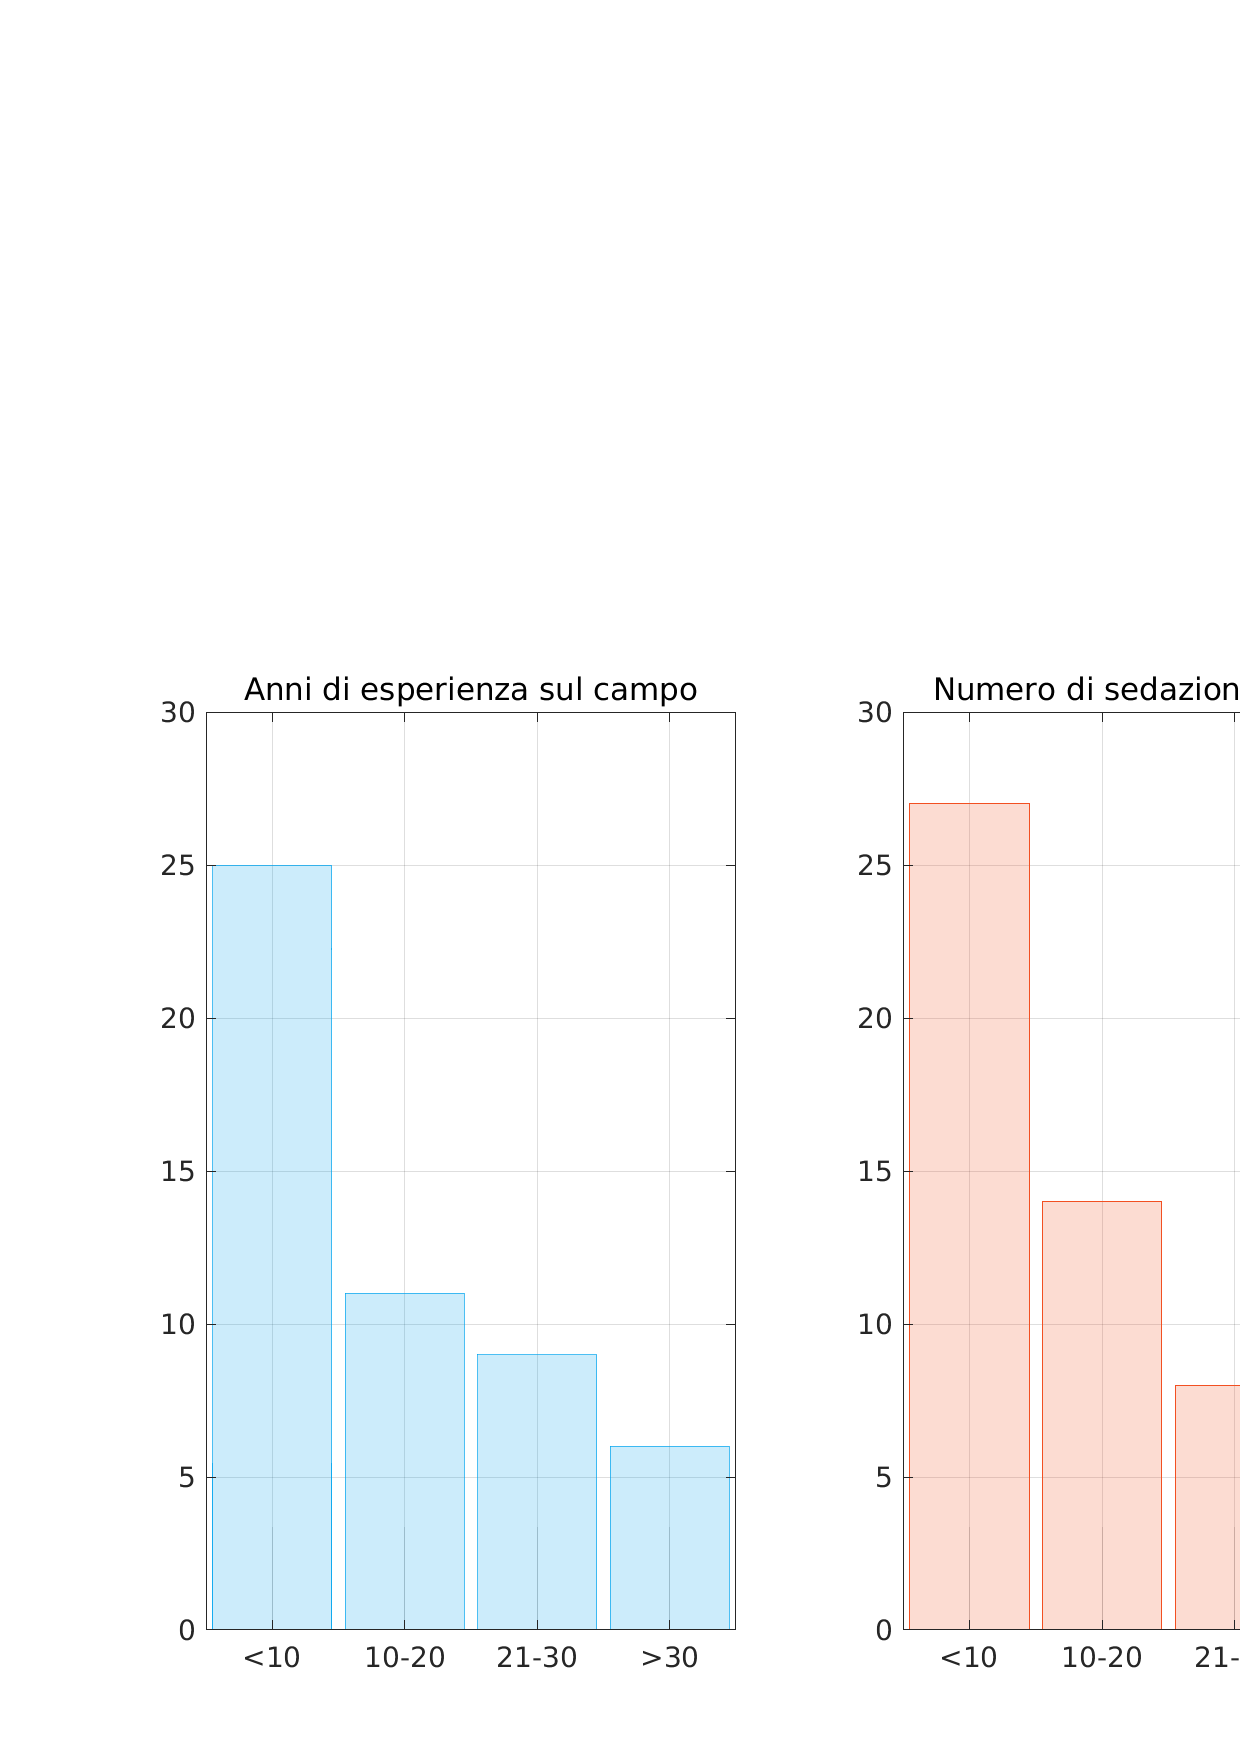
\includegraphics[width=1\textwidth]{Figure/esperienzaVSfrequenza.pdf}
    \caption{Anni di esperienza nell'ambito delle sedazioni procedurali e numero di sedazioni mensilmente assistite. Generata dal codice \ref{code:seniority-vs-experience}.}
    \label{fig:esperienzavsfrequenza}
\end{figure}

\vfill

\newpage
Come si può osservare nella figura \ref{fig:preferenze}, complessivamente il propofol è stato l'agente farmacologico più scelto dagli infermieri per le sedazioni procedurali pediatriche; infatti, 25 persone l'hanno indicato come sedativo favorito, 15 hanno scelto il midazolam, 9 la dexmedetomidina e solo 2 la ketamina. 

\begin{figure}[!ht]
    \centering
    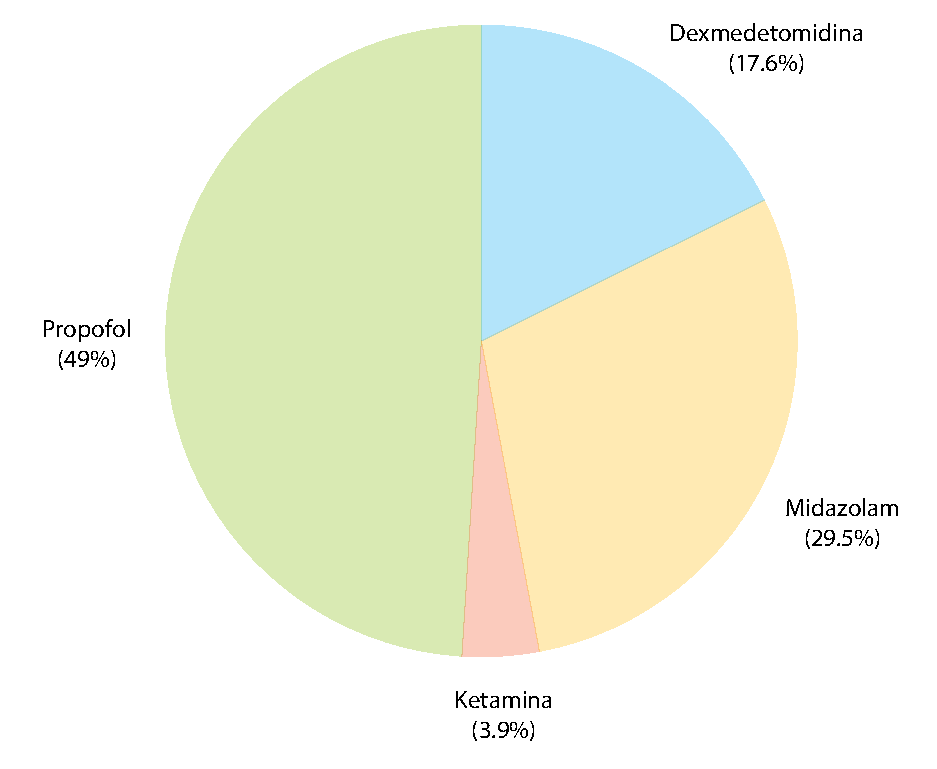
\includegraphics[width=0.7\textwidth]{Figure/preferenze.pdf}
    \caption{Farmaci preferiti dagli infermieri per le sedazioni procedurali pediatriche.}
    \label{fig:preferenze}
\end{figure}

%\vfill


\section{Percezione complessiva della qualità della sedazione}
Gli infermieri intervistati hanno dato una valutazione elevata a quasi tutti i farmaci testati: in particolare 32 partecipanti hanno attribuito un punteggio\footnote{Il grado di soddisfazione è stato misurato secondo scala \texttt{NRS}, da 0 a 10.} $\geq8$ alla qualità della sedazione con il propofol, 26 a quella con il midazolam, 23 a quella con la dexmedetomidina. I livelli di soddisfazione più bassi sono stati riscontrati con l'utilizzo della ketamina, infatti solo 8 persone hanno assegnato un punteggio $\geq8$. Nella figura \ref{fig:qualitascolorful} si possono osservare i valori della mediana, del primo e del terzo quartile relativi al livello di soddisfazione percepito dal personale infermieristico: graficamente si evince che la ketamina presenta un valore atteso significativamente inferiore al propofol, al midazolam ed alla dexmedetomidina, laddove quest'ultimi tre hanno ottenuto lo stesso risultato. Eseguendo poi il test di Kruskal-Wallis e successivamente le correzioni post test di Bonferroni e Dunn--Šidák viene dapprima rigettata, con un p--value pari a $4.34\times10^{-9}$, l'ipotesi nulla tale per cui i dati associati alla soddisfazione degli infermieri per i quattro farmaci appartengano alla stessa popolazione e viene, in secondo luogo, confermata la differenza statisticamente significativa nel confronto tra le mediane della ketamina e quelle degli altri tre sedativi, i valori di p--value sono riportati nella tabella \ref{tab:qualitatest}. 

%Si evince sia graficamente che numericamente una differenza statisticamente significativa tra le mediane dei voti attribuiti ai quattro farmaci sedativi ed analgesici testati, eseguendo il test di Kruskal-Wallis si ottiene un p--value pari a $4.34\times10^{-9}$. Nello specifico la ketamina ha mostrato un valore atteso significativamente inferiore al propofol, al midazolam ed alla dexmedetomidina, laddove quest'ultimi tre hanno ottenuto lo stesso punteggio, come descritto nella tabella \ref{tab:qualitatest}.

\vfill

\begin{figure}[!h]
    \centering
    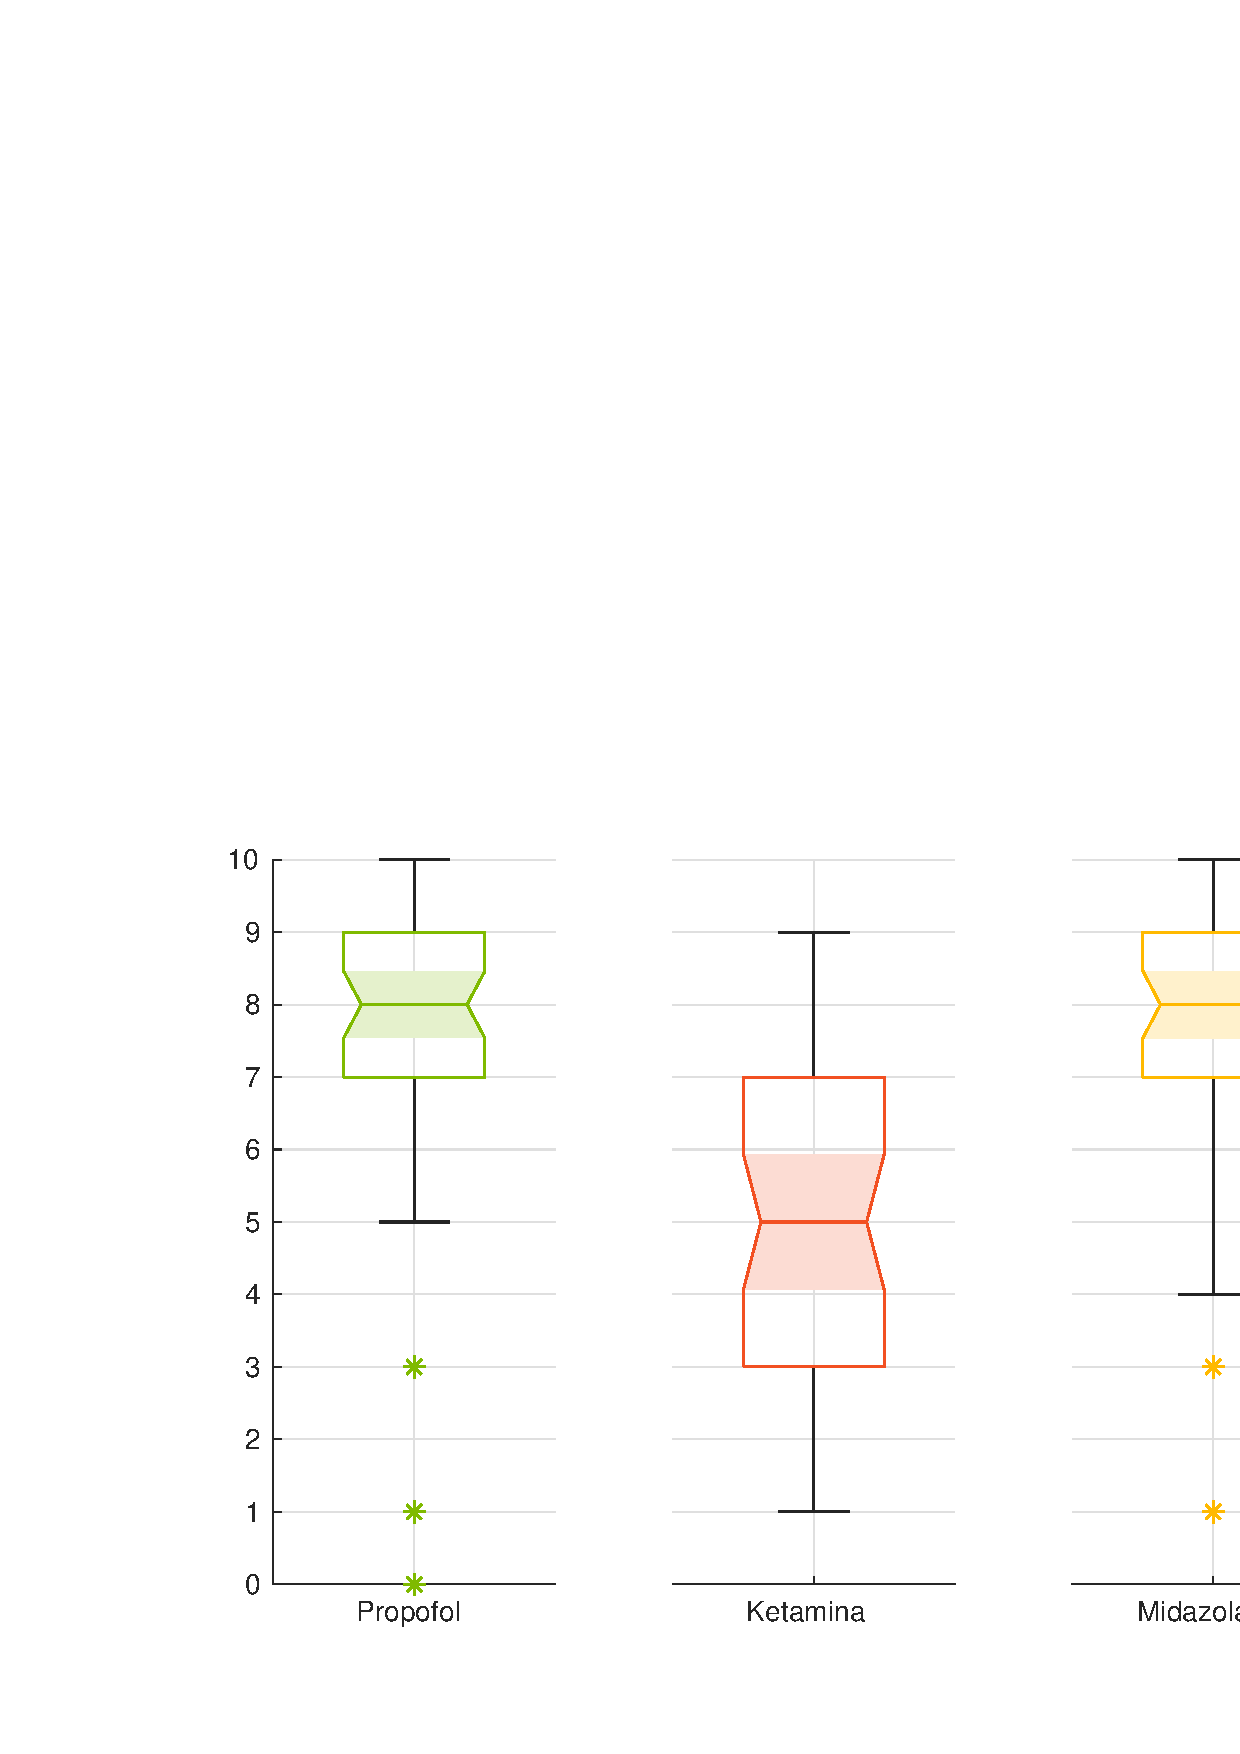
\includegraphics[width=0.95\textwidth]{Figure/qualita-colorful.pdf}
    \caption{Livello di soddisfazione percepito dagli infermieri, misurato secondo scala \texttt{NRS}, a confronto tra i quattro agenti farmacologici. Generata dal codice \ref{code:quality-global}.}
    \label{fig:qualitascolorful}
\end{figure}

\vfill\vfill


\bgroup
\def\arraystretch{1.5}
\begin{table}[!h]
    \centering
    \begin{tabular}{c|c|c|c}
         Gruppo A & Gruppo B & Bonferroni p--value & Dunn--Šidák p--value\\ \hline
       Propofol & Ketamina & $\mathbf{1.7\times10^{-8}}$ & $\mathbf{1.7\times10^{-8}}$ \\
       Propofol & Midazolam  & 1.0 & $9.7 \times 10^{-1}$\\
       Propofol & Dexmedetomidina & $6.0 \times 10^{-1}$ & $4.7 \times 10^{-1}$\\
       Ketamina & Midazolam & $\mathbf{1.4\times10^{-6}}$ & $\mathbf{1.4\times10^{-6}}$\\
       Ketamina & Dexmedetomidina & $\mathbf{3.3\times10^{-4}}$ & $\mathbf{3.3\times10^{-4}}$\\
       Midazolam & Dexmedetomidina & 1.0 & $9.3 \times 10^{-1}$\\
       
    \end{tabular}
    \caption{p--value risultanti dal confronto tra le coppie dei quattro farmaci ottenuti tramite i test di Bonferroni e di Dunn--Šidák. Generata dal codice \ref{code:quality-global}.}
    \label{tab:qualitatest}
\end{table}
\egroup

\vfill

\begin{comment}

\bgroup
\def\arraystretch{1.5}
\begin{table}[ht]
    \centering
    \begin{tabular}{|l|l|}
         Regimi farmacologici & Mediana (IQR) \\ \hline
       Propofol & 8 (7-9)  \\
       Ketamina & 5 (3-7) \\
       Midazolam & 8 (7-9) \\
       Dexmedetomidina & 8 (6-8) 
    \end{tabular}
    \caption{Valori di mediana e quartili associati alla qualità complessiva della sedazione con i quattro agenti farmacologici.}
    \label{tab:qualitased}
\end{table}
\egroup
\end{comment}


\section{Stratificazione sugli anni di esperienza e sul numero di sedazioni mensili}

Stratificando il grado di soddisfazione percepito dal personale infermieristico sugli anni di esperienza compiuti nel campo delle sedazioni procedurali non risultano differenze statisticamente significative, dal momento che i notch si sovrappongono, come graficamente visibile nella figura \ref{fig:qualitaesperienza}. Invece, analizzando la stratificazione dei punteggi di soddisfazione relativi ai quattro farmaci sul numero di sedazioni mensilmente effettuate si osserva una differenza significativa tra le mediane, in particolare si nota che il voto associato al propofol aumenta con il numero di procedure assistite ogni mese dagli infermieri. Questo dato risulta graficamente evidente dalla non sovrapposizione dei notch nella figura \ref{fig:qualitafrequenza}. 

%in particolare, gli infermieri che prendono parte a più di 20 sedazioni al mese risultano maggiormente soddisfatti delle sedazioni con il propofol rispetto a coloro che partecipano a un minor numero di sedazioni. Questo dato risulta graficamente evidente dalla non sovrapposizione dei relativi notch. 


%si osserva un incremento della soddisfazione relativa alla sedazione con il propofol con il numero di sedazioni mensili. non risultano differenze statisticamente significative, laddove i notch non si sovrappongono, come graficamente visibile nelle figure \ref{fig:qualitaesperienza} e \ref {fig:qualitafrequenza}.


\vfill
\begin{figure}[ht]
    \centering
    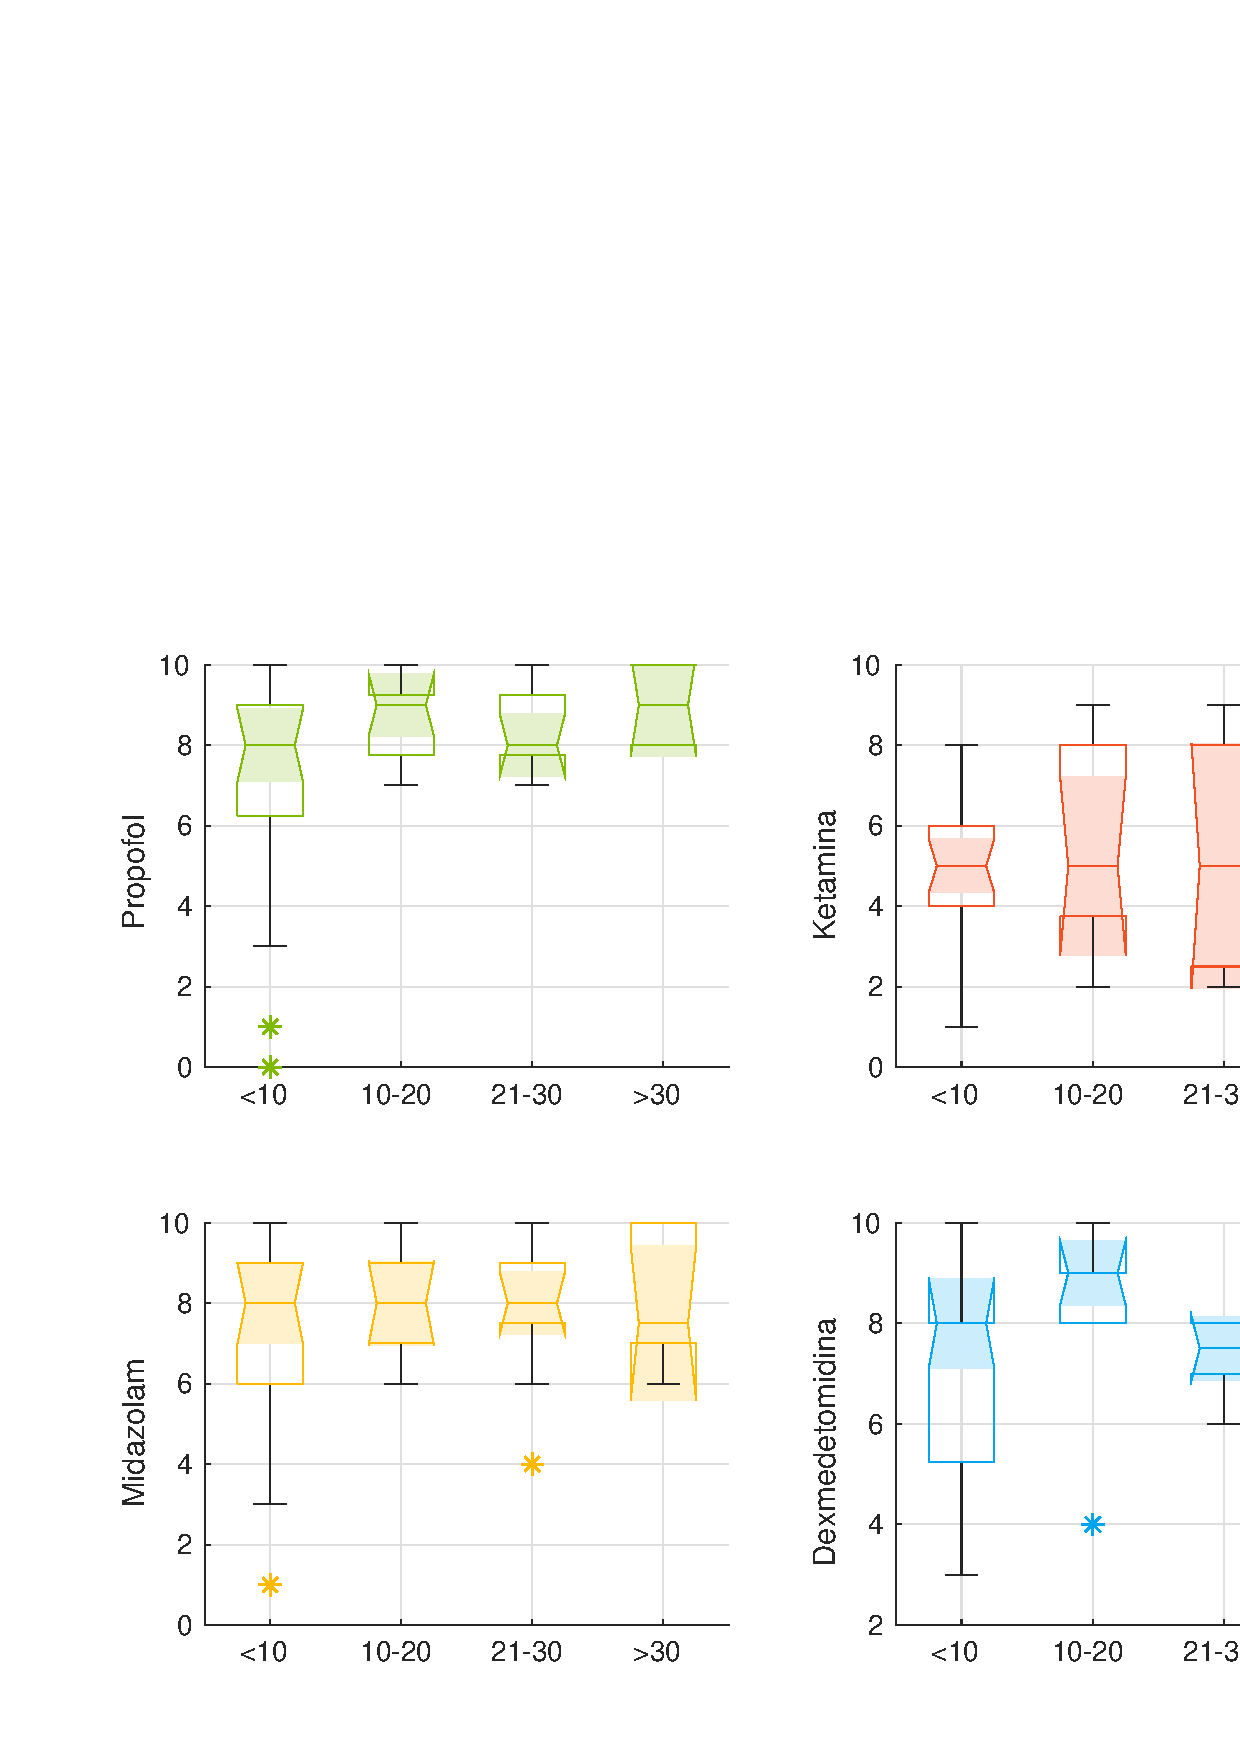
\includegraphics[width=0.95\textwidth]{Figure/qualita-strat-esperienza.pdf}
    \caption{Livello di soddisfazione, associato ai diversi agenti farmacologici, stratificato sugli anni di esperienza dei partecipanti nell'ambito delle sedazioni procedurali. Generata dal codice \ref{code:quality-strati}.}
    \label{fig:qualitaesperienza}
\end{figure}

\vfill
\begin{figure}[!h]
    \centering
    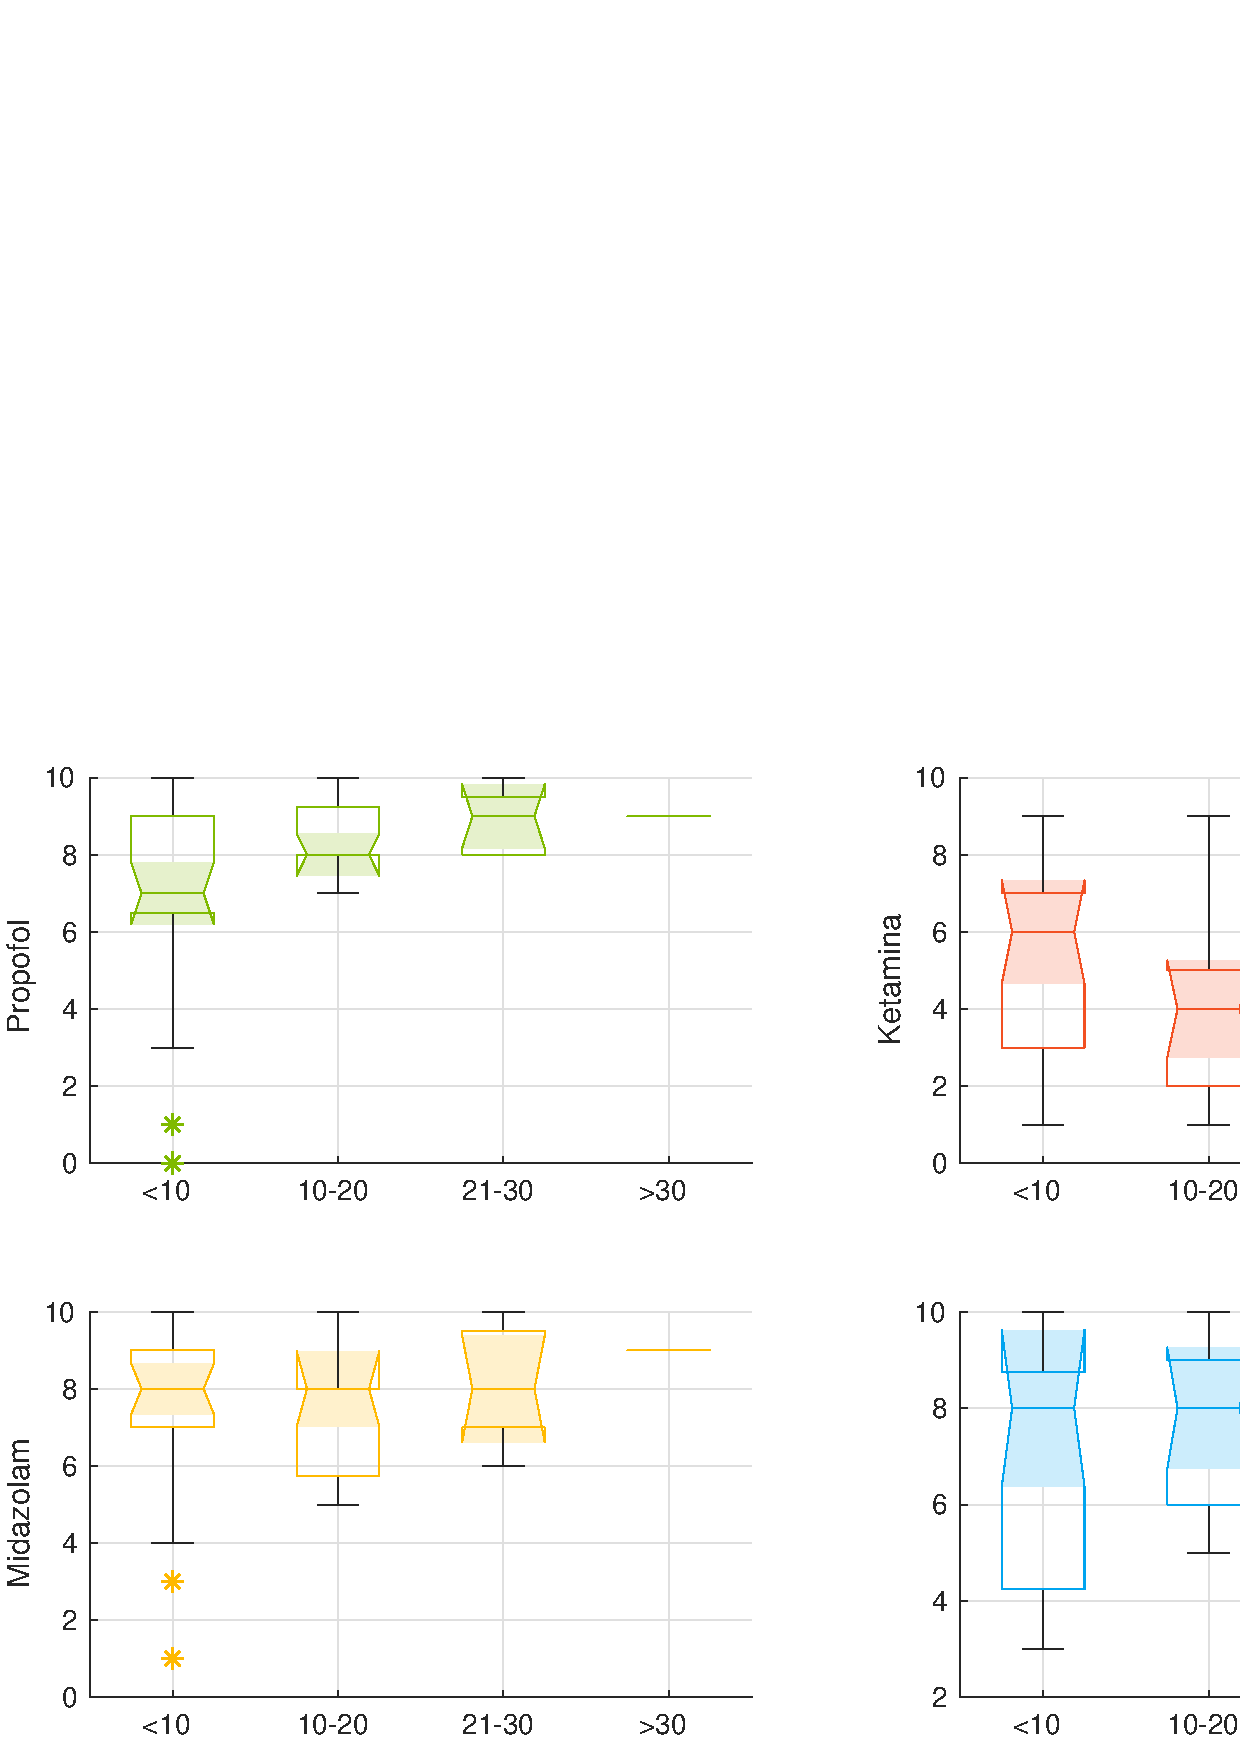
\includegraphics[width=0.95\textwidth]{Figure/qualita-strat-frequenza.pdf}
    \caption{Livello di soddisfazione, associato ai diversi agenti farmacologici, stratificato sul numero di sedazioni mensilmente assistite dagli intervistati. Generata dal codice \ref{code:quality-strati}.}
    \label{fig:qualitafrequenza}
\end{figure}

\vfill
\newpage

\vfill
\section{Grado di sicurezza percepito ed effetti avversi}

Il livello di sicurezza percepito durante la sedazione è risultato complessivamente elevato per tutti i farmaci testati, con una differenza statisticamente poco significativa tra i quattro gruppi: il test di Kruskal-Wallis ha restituito un valore di p--value pari a 0.04. In particolare, effettuando la correzione di Bonferroni e la correzione di Dunn--Šidák, quindi, confrontando le mediane dei dati relativi alla sicurezza percepita dagli infermieri per i quattro farmaci, è emersa una superiorità del midazolam rispetto alla dexmedetomidina. Tuttavia, tale differenza si può considerare statisticamente poco significativa, in quanto i valori dei p--value si trovano appena al di sotto della soglia $\alpha$ di significatività. I risultati ottenuti\footnote{I dati statistici sono stati ricavati attribuendo un valore pari a 0 alla risposta \emph{per niente}, pari a 1 a \emph{poco}, pari a 2 a \emph{molto}.} sono rappresentati nella figura \ref{fig:sicurezza1} e i valori di p--value per ogni test effettuato sono riportati nella tabella \ref{tab:sicurezzatest}.

\vfill

\begin{figure}[!h]
    \centering
    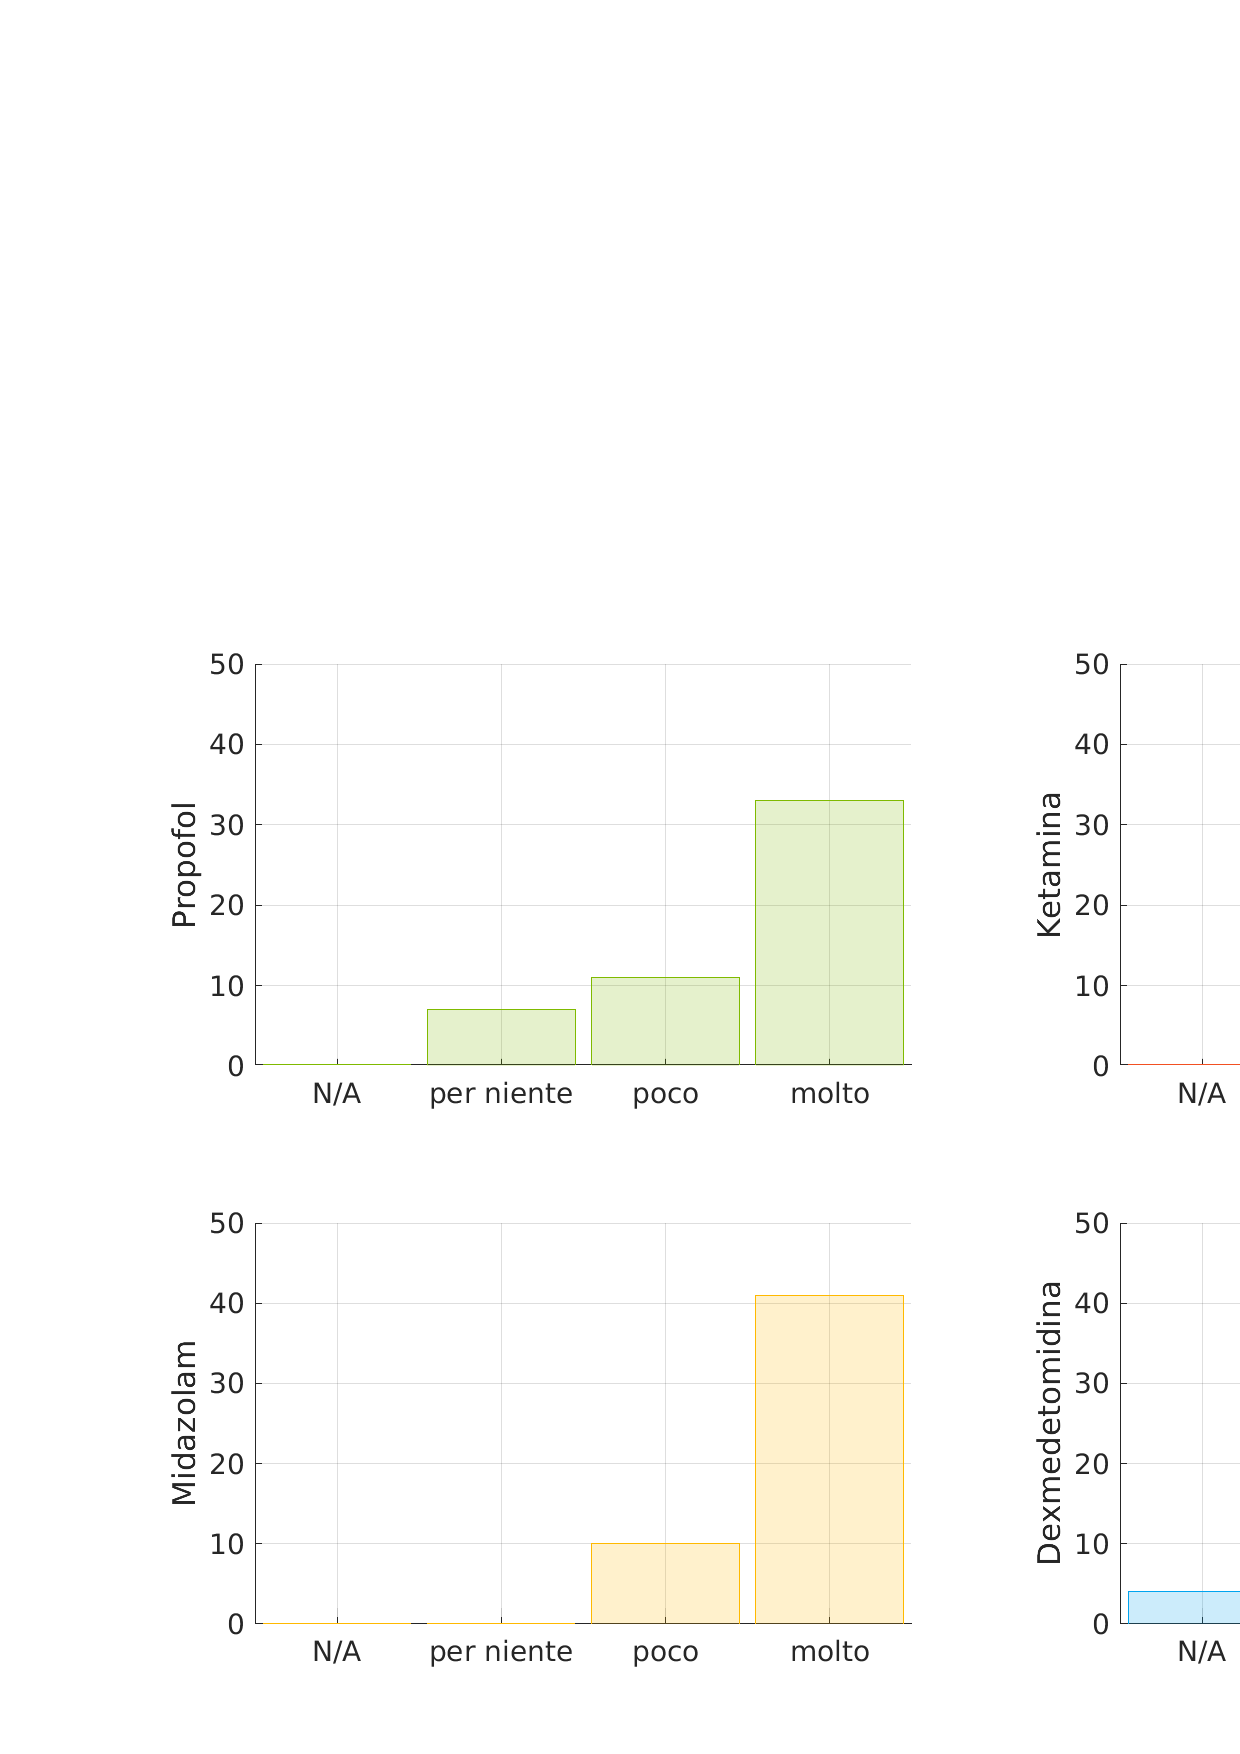
\includegraphics[width=1\textwidth]{Figure/sicurezza-istogrammi.pdf}
    \caption{Risposte alla domanda "Quanto ti senti sicuro durante la sedazione con i seguenti farmaci?". Generata dal codice \ref{code:safety}.}
    \label{fig:sicurezza1}
\end{figure}

\vfill

\newpage

\bgroup
\def\arraystretch{1.5}
\begin{table}[!h]
    \centering
    \begin{tabular}{c|c|c|c}
         Gruppo A & Gruppo B & Bonferroni p--value & Dunn--Šidák p--value\\ \hline
       Propofol & Ketamina & 1.0 & $9.9 \times 10^{-1}$ \\
       Propofol & Midazolam  & $2.9 \times 10^{-1}$ & $2.6 \times 10^{-1}$\\
       Propofol & Dexmedetomidina & 1.0 & $9.8 \times 10^{-1}$\\
       Ketamina & Midazolam & $1.7\times10^{-1}$ & $1.5\times10^{-1}$\\
       Ketamina & Dexmedetomidina & 1.0 & $9.9\times10^{-1}$\\
       Midazolam & Dexmedetomidina & $\mathbf{4.9 \times 10^{-2}}$ & $\mathbf{4.8 \times 10^{-2}}$\\
       
    \end{tabular}
    \caption{p--value ottenuti tramite i test di Bonferroni e di Dunn--Šidák: confronto a coppie dei quattro farmaci per valutarne il profilo di sicurezza come percepito dagli infermieri. Generata dal codice \ref{code:safety}.}
    \label{tab:sicurezzatest}
\end{table}
\egroup

\vfill

\begin{comment}

di mediana e IQR descritti nella tabella \ref{tab:sicurezzased}.

\vfill

%(Kruskal-Wallis p--value 0.08)
\bgroup
\def\arraystretch{1.5}
\begin{table}[ht]
    \centering
    \begin{tabular}{|l|l|}
         Regimi farmacologici & Mediana (IQR) \\ \hline
       Propofol & 10 (6--10)  \\
       Ketamina & 10 (6--10) \\
       Midazolam & 10 (10--10) \\
       Dexmedetomidina & 10 (6--10) 
    \end{tabular}
    \caption{Valori di mediana e quartili associati alla sicurezza percepita durante la sedazione con i quattro agenti farmacologici. Generata dal codice \ref{code:safety}.}
    \label{tab:sicurezzased}
\end{table}
\egroup
\end{comment}

\vfill


\begin{figure}[!h]
    \centering
    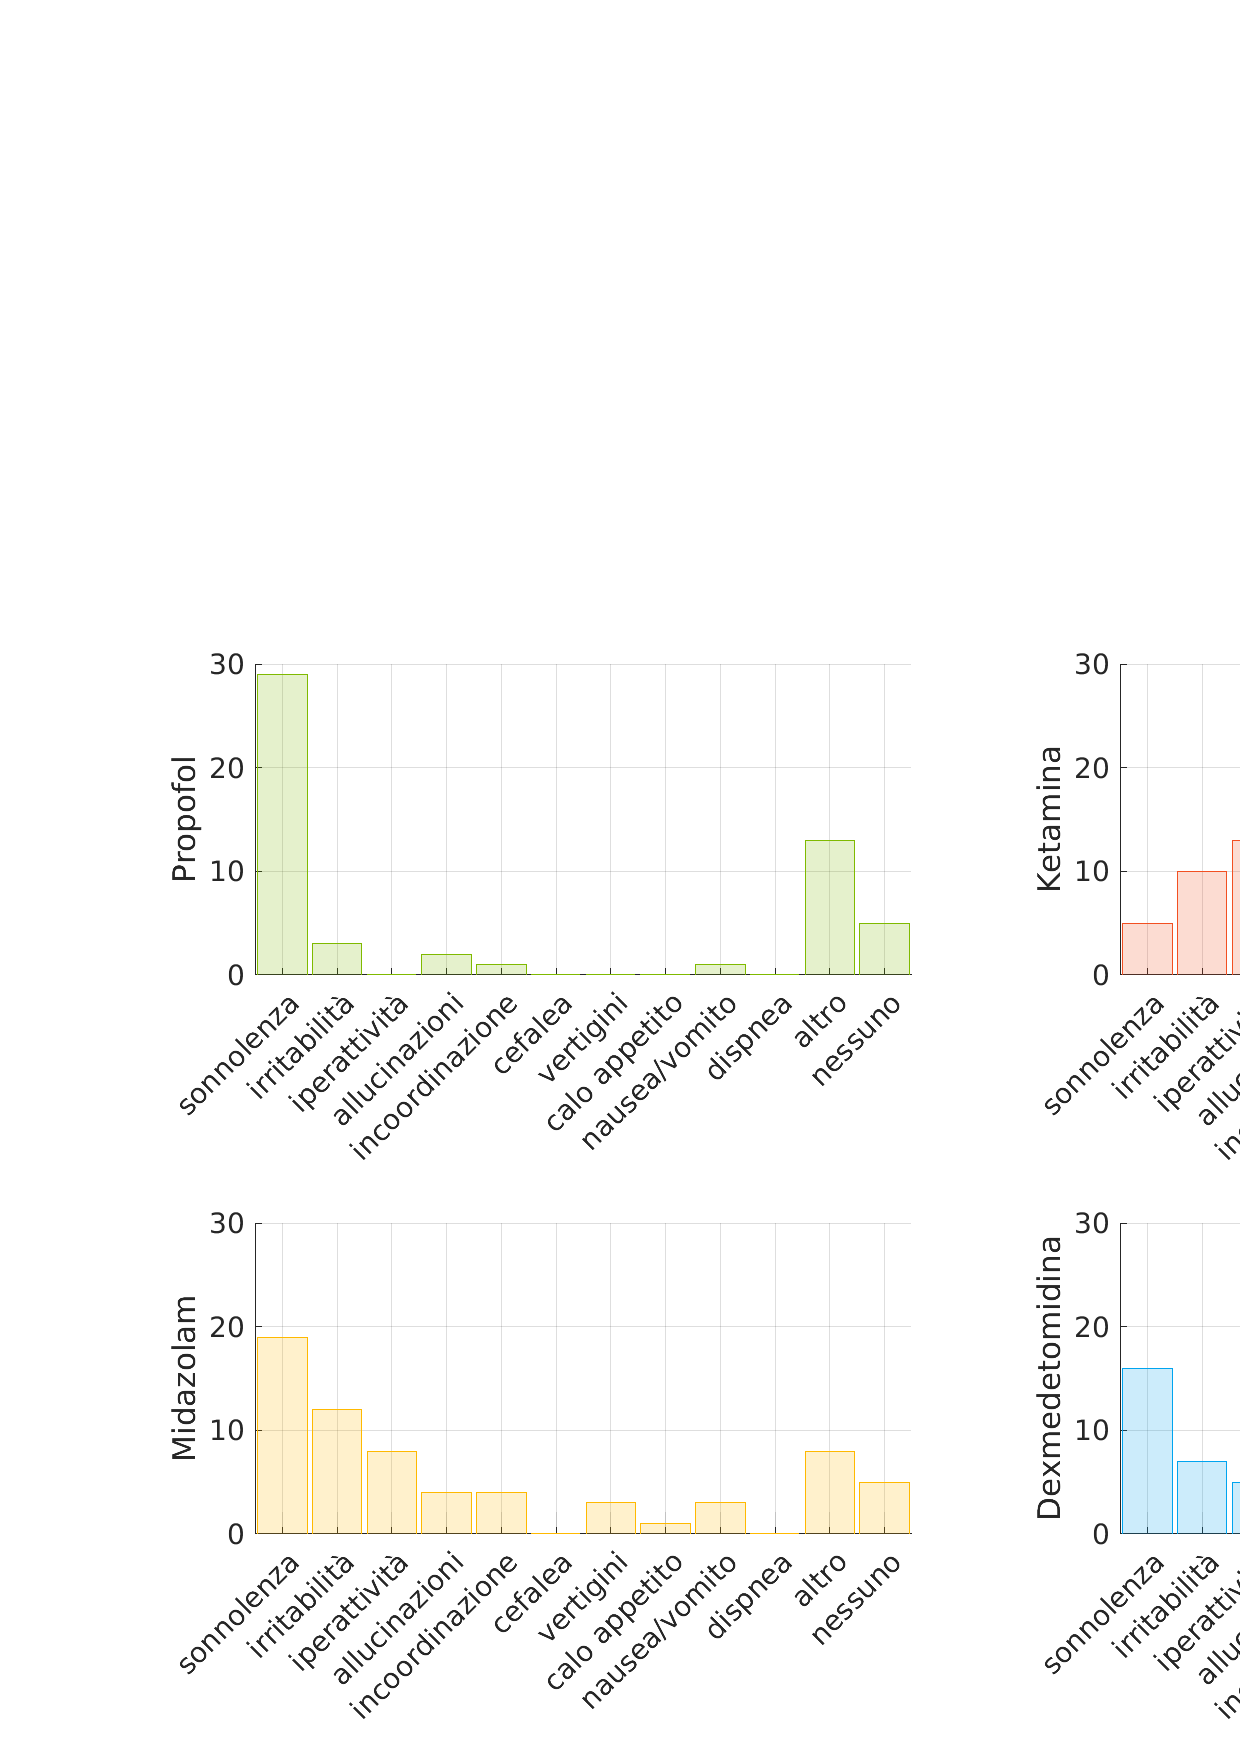
\includegraphics[width=1\textwidth]{Figure/effetti-avversi.pdf}
    \caption{Gli effetti avversi più frequentemente riscontrati dagli infermieri con i quattro agenti farmacologici testati. Generata dal codice \ref{code:adverse-effects-incidence}.}
    \label{fig:sicurezza}
\end{figure}

\vfill

Le reazioni avverse più comunemente osservate dal personale intervistato per i quattro farmaci valutati nello studio sono rappresentate nella figura \ref{fig:sicurezza}. Secondo il parere infermieristico, la sola sonnolenza è più frequentemente associata alla sedazione con il propofol; oltre ad essa l'irritabilità, l'iperattività o l'irrequietezza sono spesso correlate all'utilizzo del midazolam e della dexmedetomidina; invece la ketamina presenta gli effetti collaterali più spiacevoli: allucinazioni, nausea e vomito, oltre nuovamente ad iperattività, irrequietezza ed irritabilità.

\begin{comment}

\bgroup
\def\arraystretch{1.5}
\begin{table}[!h]
    \centering
    \begin{tabular}{p{0.18\textwidth} p{0.12\textwidth} p{0.12\textwidth} p{0.12\textwidth} p{0.16\textwidth}}
  & \footnotesize{Propofol} & \footnotesize{Ketamina} & \footnotesize{Midazolam} & \footnotesize{Dexmedetomidina}\\ \hline
    \footnotesize{Sonnolenza} & \footnotesize29 & \footnotesize5 & \footnotesize19 & \footnotesize16\\ \hline
    \footnotesize{Irritabilità} & \footnotesize3 & \footnotesize10 & \footnotesize12 & \footnotesize7\\ \hline
    \footnotesize{Iperattività} & \footnotesize0 & \footnotesize13 & \footnotesize8 & \footnotesize5\\ \hline
    \footnotesize{Allucinazioni} & \footnotesize2 & \footnotesize21 & \footnotesize4 & \footnotesize2\\ \hline
    \footnotesize{Incoordinazione} & \footnotesize0 & \footnotesize6 & \footnotesize4 & \footnotesize2\\ \hline
    \footnotesize{Cefalea} & \footnotesize0 & \footnotesize0 & \footnotesize0 & \footnotesize0\\ \hline
    \footnotesize{Vertigini}  & \footnotesize0 & \footnotesize2 & \footnotesize3 & \footnotesize1\\ \hline
    \footnotesize{Calo appetito} & \footnotesize0 & \footnotesize7 & \footnotesize1 & \footnotesize1\\ \hline
    \footnotesize{Nausea/vomito} & \footnotesize1 & \footnotesize18 & \footnotesize3 & \footnotesize3\\ \hline
    \footnotesize{Dispnea} & \footnotesize0 & \footnotesize0 & \footnotesize0 & \footnotesize0\\ \hline
    \footnotesize{Nessuno} & \footnotesize12 & \footnotesize2 & \footnotesize6 & \footnotesize7\\ \hline
    \footnotesize{N/A} & \footnotesize5 & \footnotesize6 & \footnotesize12 & \footnotesize5\\ 

    \end{tabular}
    \caption{Opinione degli infermieri riguardo la frequenza degli effetti avversi con i quattro regimi farmacologici.}
    \label{tab:effavv}
\end{table}
\egroup

\end{comment}


\begin{figure}[!h]
    \centering
    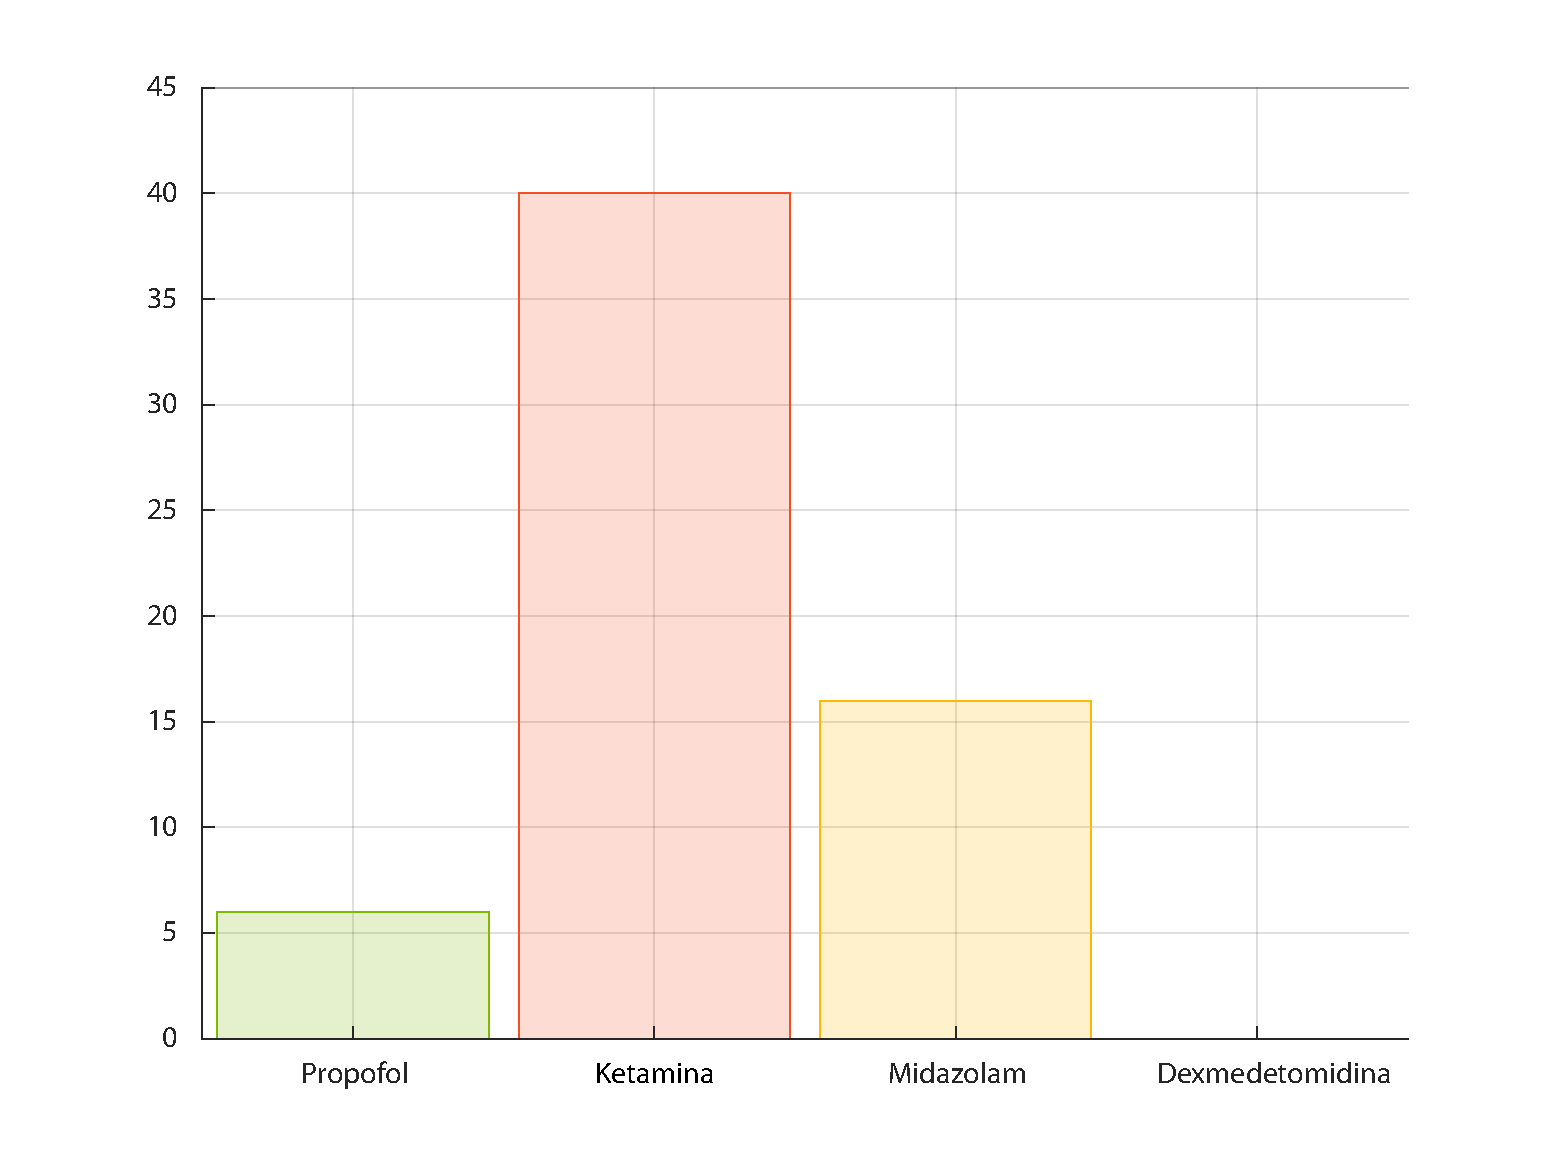
\includegraphics[width=0.9\textwidth]{Figure/rescue (1).pdf}
    \caption{Risposte degli infermieri alla domanda "Per quali di queste sedazioni è spesso necessario somministrare al risveglio un farmaco \emph{rescue} o sintomatico?". Generata dal codice \ref{code:rescue}.}
    \label{fig:rescue}
\end{figure}

Inoltre, la necessità di utilizzare farmaci \emph{rescue}, quali antiemetici per la nausea ed il vomito, flumazenil per il \emph{midazolam-induced paradox phenomenon} o infusione di soluzioni contenenti glucosio per evitare eventuali ipoglicemie, soprattutto nei pazienti più piccoli, in caso di tempi di risveglio prolungati, è stata associata da 40 infermieri alla sedazione con ketamina, da 16 a quella con midazolam e da 5 a quella con propofol, come evidenziato nella figura \ref{fig:rescue}.


\section{Elementi che influenzano il grado di soddisfazione}

Al fine di comprendere al meglio i motivi alla base delle risposte riportate dagli infermieri aderenti allo studio, è stato chiesto loro di indicare quali aspetti hanno influenzato maggiormente il loro giudizio sulla qualità complessiva. La maggior parte ha riferito che gli elementi che hanno pesato di più sul grado di soddisfazione globale della sedazione sono stati: la qualità del risveglio, la presenza di effetti avversi e l'insoddisfazione del bambino e della famiglia. Invece, il tipo di farmaco utilizzato, la via di somministrazione, il tempo di risveglio, la necessità di ricorrere a farmaci \emph{rescue} e l'impegno infermieristico sono fattori che hanno influito marginalmente alla valutazione finale.

\begin{figure}[!h]
    \centering
    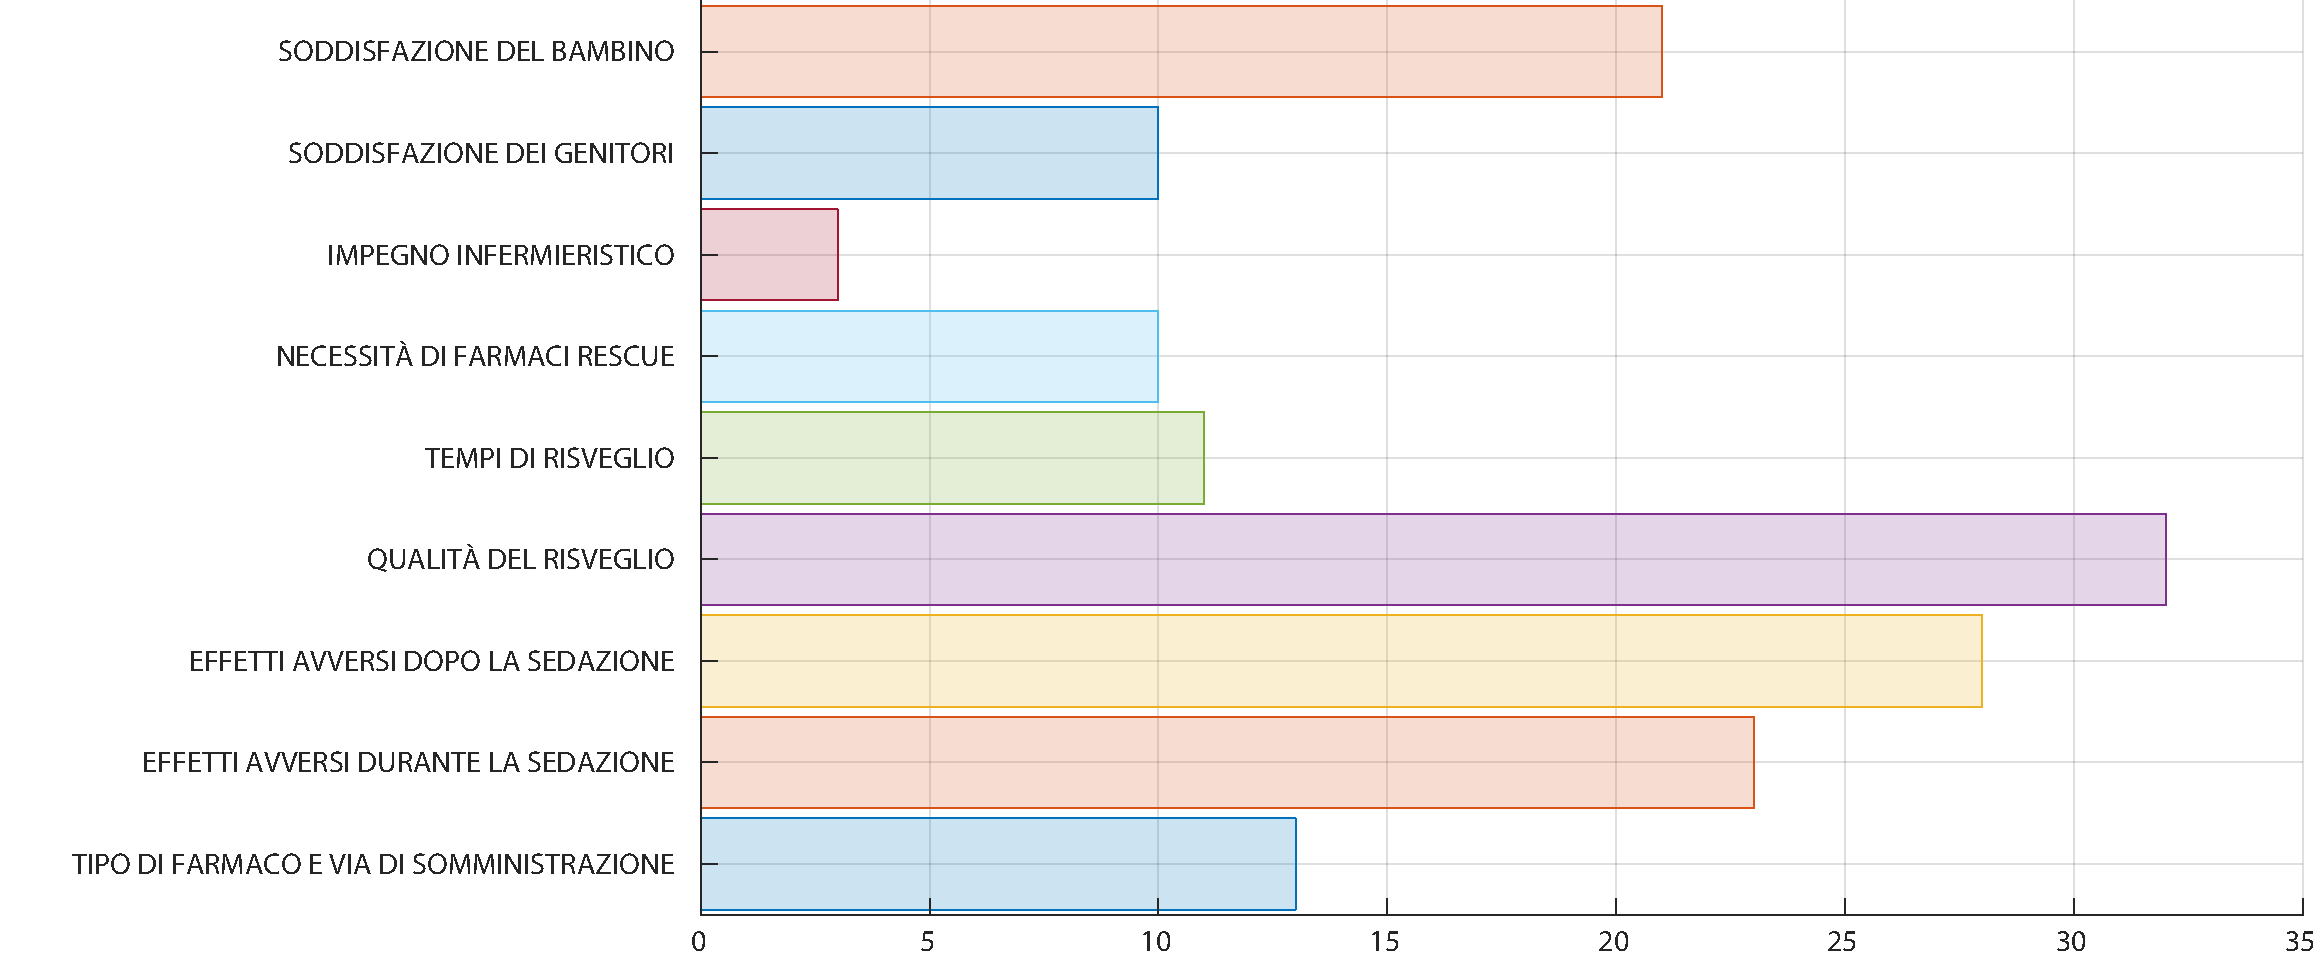
\includegraphics[width=1\textwidth]{Figure/soddisfazione-globale (1).pdf}
    \caption{Fattori che hanno influenzato il grado di soddisfazione complessivo degli infermieri. Generata dal codice \ref{code:satisfaction}.}
    \label{fig:soddglobale}
\end{figure}

\newpage
Oltre a ciò, è stato domandato quanto l'incidenza dei possibili effetti collaterali pesi negativamente sul livello di soddisfazione derivato dalla scelta dei diversi sedativi ed analgesici: è emerso che l'insorgenza di distress respiratorio costituisce l'elemento che influisce maggiormente sul giudizio degli infermieri; mentre la manifestazione di nausea o vomito, vertigini, allucinazioni, iperattività od irritabilità esercita un'influenza moderata; infine, la presenza di sonnolenza, incoordinazione motoria, cefalea e alterazioni dell'appetito risulta meno rilevante ai fini del livello di soddisfazione globale percepito (cfr. fig. \ref{fig:influenzaeffetti} e tab. \ref{tab:effavv2}). 

\vfill

\begin{figure}[!ht]
    \centering
    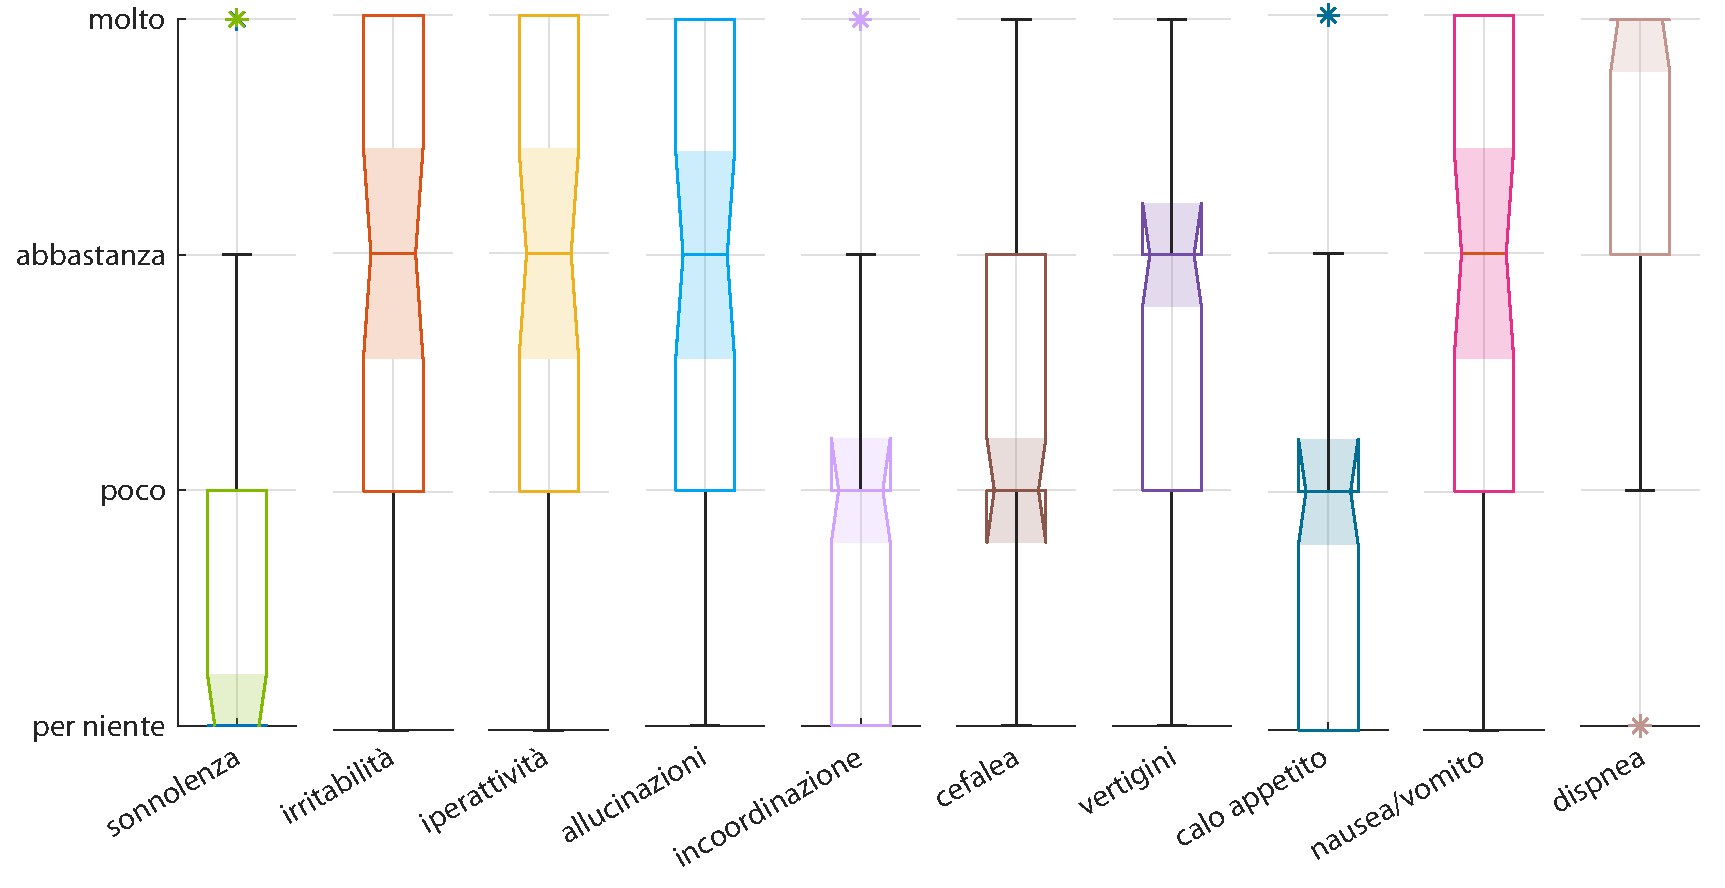
\includegraphics[width=1\textwidth]{Figure/influenza-effetti.pdf}
    \caption{Risposte alla domanda "Quanto i seguenti effetti collaterali riducono la tua soddisfazione in merito alla sedazione procedurale?". Generata dal codice \ref{code:adverse-effects-perception}.}
    \label{fig:influenzaeffetti}
\end{figure}

\newpage

\bgroup
\def\arraystretch{1.5}
\begin{table}[!h]
    \centering
    \begin{tabular}{p{0.18\textwidth} p{0.17\textwidth} p{0.17\textwidth} p{0.17\textwidth} p{0.17\textwidth}}
  & \footnotesize{Nessuna influenza} & \footnotesize{Poca influenza} & \footnotesize{Modesta influenza} & \footnotesize{Molta influenza}\\ \hline
    \footnotesize{Sonnolenza} & \footnotesize29 & \footnotesize19 & \footnotesize1 & \footnotesize2\\ \hline
    \footnotesize{Irritabilità} & \footnotesize12 & \footnotesize10 & \footnotesize14 & \footnotesize15\\ \hline
    \footnotesize{Iperattività} & \footnotesize8 & \footnotesize13 & \footnotesize16 & \footnotesize14\\ \hline
    \footnotesize{Allucinazioni} & \footnotesize9 & \footnotesize8 & \footnotesize17 & \footnotesize17\\ \hline
    \footnotesize{Incoordinazione} & \footnotesize15 & \footnotesize25 & \footnotesize7 & \footnotesize4\\ \hline
    \footnotesize{Cefalea} & \footnotesize12 & \footnotesize18 & \footnotesize16 & \footnotesize5\\ \hline
    \footnotesize{Vertigini}  & \footnotesize9 & \footnotesize16 & \footnotesize18 & \footnotesize8\\ \hline
    \footnotesize{Calo appetito} & \footnotesize22 & \footnotesize25 & \footnotesize2 & \footnotesize2\\ \hline
    \footnotesize{Nausea/vomito} & \footnotesize6 & \footnotesize13 & \footnotesize16 & \footnotesize16\\ \hline
    \footnotesize{Dispnea} & \footnotesize6 & \footnotesize3 & \footnotesize7 & \footnotesize35\\ \hline

    \end{tabular}
    \caption{Influenza degli effetti avversi sulla valutazione infermieristica.}
    \label{tab:effavv2}
\end{table}
\egroup



\section{Preferenze relative alle vie di somministrazione}

Le vie di somministrazione favorite dagli infermieri sono, in ordine di preferenza: via endovenosa (scelta da 28 persone -- 55$\%$), via orale più intranasale (15 -- 29.5$\%$), via intranasale (7 -- 13.5$\%$) e via intramuscolare (1 -- 2$\%$). Inoltre, 40 infermieri (78.4$\%$) vorrebbero che un accesso venoso venisse posizionato abitualmente ed indiscriminatamente in tutti i bambini, mentre 11 (21.6$\%$) desiderano che sia inserito almeno nei casi più difficili, ad esempio nei pazienti con condizioni genetiche note, autismo, ritardo psicomotorio o un alto DIVA score. Nessun infermiere ha risposto che preferirebbe non venisse mai applicato il cateterismo venoso periferico. 

\begin{figure}[!h]
    \centering
    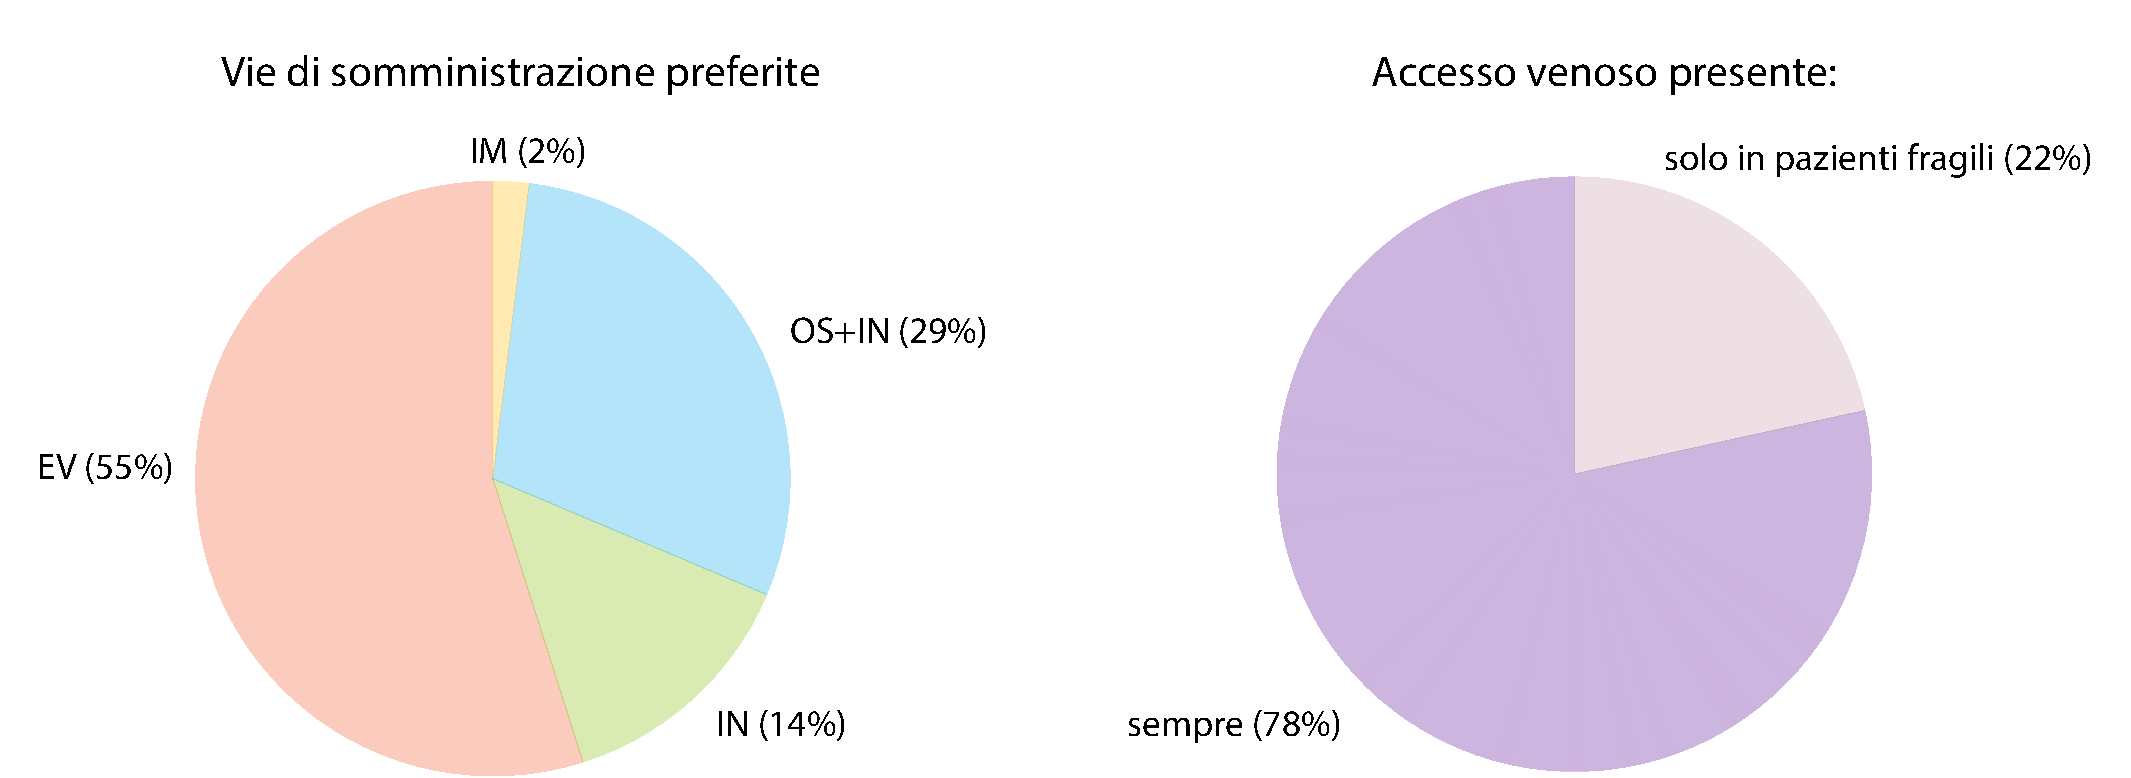
\includegraphics[width=1\textwidth]{Figure/sommicrosoftchiaro.pdf}
    \caption{Vie di somministrazione più apprezzate dagli infermieri per la sedazione procedurale e preferenze relative alla presenza o meno dell'accesso venoso.}
    \label{fig:viedisomm}
\end{figure}

\newpage

\section{Importanza dell'approccio non farmacologico}

Le tecniche di distrazione attuate prima e durante le sedazioni procedurali sono state giudicate molto importanti da parte di 31 infermieri (60.8$\%$), importanti da 7 (13.7$\%$), poco rilevanti da 9 (17.6$\%$) e non importanti da 4 (7.9$\%$).

\bigskip

\begin{figure}[!h]
    \centering
    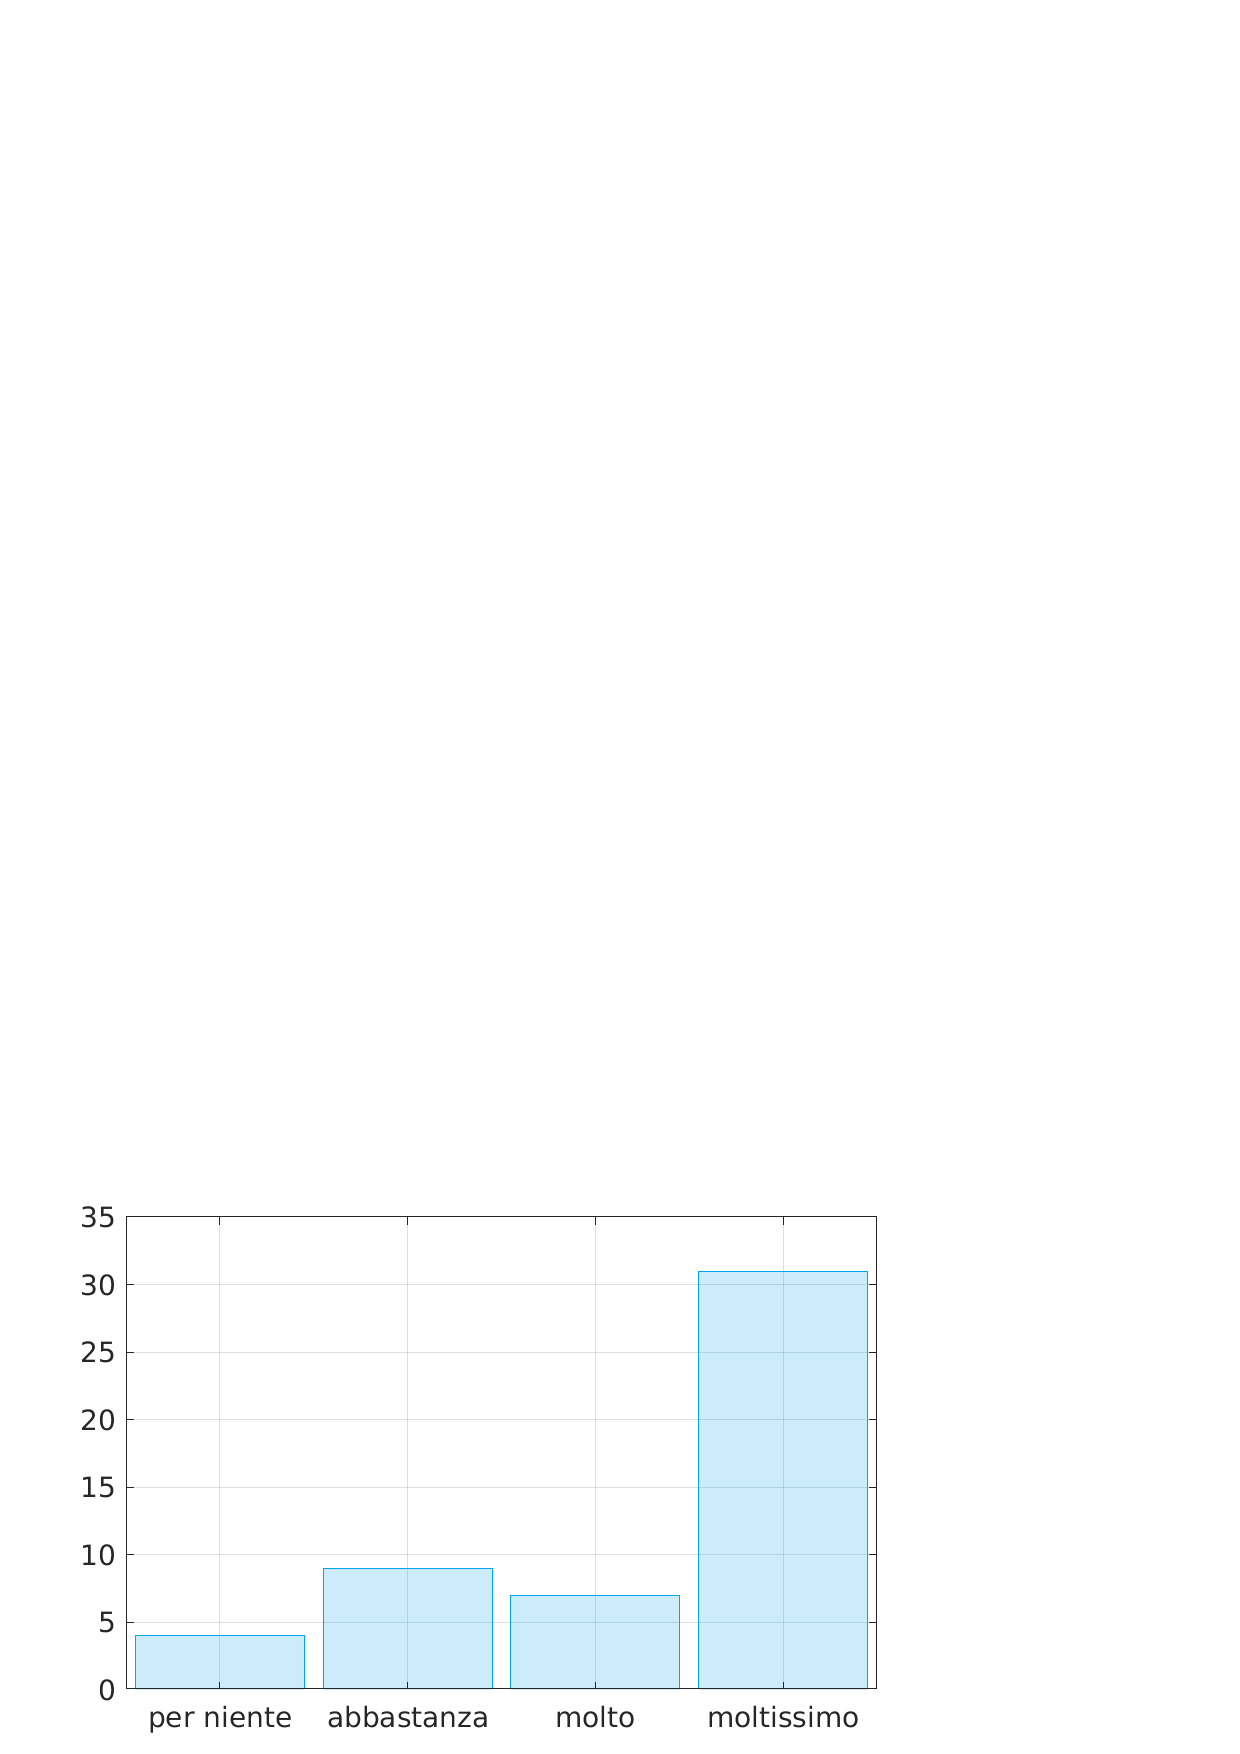
\includegraphics[width=0.7\textwidth]{Figure/distrazione.pdf}
    \caption{Risposte alla domanda "Quanto ritieni utile l’utilizzo di tecniche di distrazione nei bambini per l’esecuzione di procedure non dolorose/minimamente dolorose?". Generata dal codice \ref{code:misdirection-techniques}.}
    \label{fig:distrazione}
\end{figure}

\section{Suggerimenti per migliorare lo standard di cura attuale}

In conclusione al questionario, è stata data la possibilità di esporre eventuali modifiche che ciascun partecipante attuerebbe nella propria Unità Operativa rispetto agli attuali standard di analgosedazione. A tal proposito è emerso che la maggior parte degli infermieri vorrebbe che venissero realizzati con maggior frequenza dei corsi di formazione ed aggiornamento, inoltre è stato suggerito di implementare ulteriormente l'approccio non farmacologico e di migliorare la qualità della comunicazione tra personale medico ed infermieristico. 